%!TEX root = ../main.tex

\chapter{Introduction}
\label{chap:introduction}

\begin{picture}(0,0)
\put(190,50){\hbox{
\includegraphics[width=4.2cm, angle=-5, trim=4 4 4 4, clip]{ferris/book}}}
\end{picture}
\vspace{-1cm}

Whether communicating with an API, reading configuration files, or using a static dataset, most modern programs at some point have to interact with external data sources. And with the rise of micro-services it is not uncommon to have to access data from many such external data sources in a single program. When programmers write code that accesses external data in a statically typed programming language, they are often faced with a dilemma between convenience and type-safety. For type-safe access to external data, significant boiler-plate in the form of code with abundant checks or a large amount of custom types must usually be written. While approaches that avoid this boiler-plate often abandons many of the benefits of static types.

In the programming language F\#, a concept called type providers has been proposed as a solution to this problem by having compiler support for libraries with the capability to generate custom types, based on the external data, at compile time. With this method, a type provider offers access to external, potentially complex resources, in a way that is both convenient and type-safe.

This thesis presents «json_typegen», a project which aims to show the feasibility of similar solutions in the Rust programming language. The project uses compile-time metaprogramming, along with alternative interfaces to the same code generation implementation, to achieve convenient, type-safe access to data in the JSON data format, in a way similar to the type providers of F\#. The presented project provides support for the very common JSON format, but the approach, and much of the actual code used by «json_typegen», can be applied to create similar tools for other data formats and sources.

In this introductory chapter we will look at the background for the «json_typegen» project. First, in section~\ref{sec:rust-intro}, we will look at the Rust programming language. Then, in section~\ref{sec:json}, we will look at the JSON data interchange format, and the challenges associated with accessing data in JSON from statically typed programming languages, and Rust in particular. Finally, in section~\ref{sec:type-providers} we will look at how these challenges have been attempted solved with type providers in the programming language F\#.

In chapter~\ref{chap:project-presentation}, the project and its interfaces is presented in detail. And in chapter~\ref{chap:code-generation} we will look at how the code inference and code generation used in the project works, and ways in which it could be extended.

\section{The Rust programming language}
\label{sec:rust-intro}

The project presented in the thesis, «json_typegen», creates types for programs written in the Rust programming language, and is itself written in Rust. The Rust programming language is a modern, open source programming language with C-like surface syntax. It is a statically typed language with type inference, with a focus on memory safety and zero-cost abstractions.

Rust does not use a garbage collector and the core library can be used without access to heap allocation. This allows Rust to be used for what is often referred to as \say{systems programming}, e.g. for writing drivers, operating systems and code for microcontrollers. Spaces which has so far been occupied mainly by C and \cpp\footnote{There are \emph{some} other languages that can be said to compete in this area, like Ada, Objective-C and D. I won't go into the details of how these languages compare to Rust, but for various reasons \cpp\ is the main competitor and point of comparison for most use cases.}. Rust tries to combine the low-level control of these languages with modern syntax and an advanced type system that statically prevents whole classes of memory safety issues \cite{the-rust-language}.

While the basic syntax of Rust can be said to be C-like it also has a lot of functionality and syntax reminiscent of functional languages and in particular languages of the ML-family. Features such as closures, pattern matching and monadic error handling are available and a significant part of idiomatic Rust code.

What follows is a very basic introduction to the parts of Rust we need to talk about in this thesis. Many of Rusts more advanced language features are not necessary to understand the basic concepts of this thesis, and are as such not explained here. For more details on the language features of Rust, see \href{https://doc.rust-lang.org/book/}{the Rust book}\footnote{\url{https://doc.rust-lang.org/book/}}.

\subsection{Structs}

\begin{listing}[ht!]
\begin{minted}{rust}
struct Person {
    name: String,
    age: i64,
}
\end{minted}
\caption{A basic Rust struct}
\label{lst:struct}
\end{listing}

The primary language construct for complex types in Rust are structs. A struct declaration, as shown in Listing~\ref{lst:struct}, is a sequence of field names, along with their types. Structs are product types and are analogous to records in some languages. Rust does not have classes or objects, and is not object oriented in the classical sense. In other words is there no inheritance between structs, and polymorphism in Rust is instead supported by other language features, such as enumerated types, and traits.

\subsection{Enums}

\begin{listing}[ht!]
\begin{minted}{rust}
enum Option<T> {
    None,
    Some(T),
}
\end{minted}
\caption{The enumerated type ‹Option› in Rust}
\label{lst:enum}
\end{listing}

An enum in Rust is a data type that is one alternative from a number of variants, i.e. an enumerated type, sum type or union. A declaration of an enum, as seen in Listing~\ref{lst:enum} is given as a list of variant names, used as constructors. Each variant can optionally carry some associated data.

Rust supports pattern matching on enum types and verifies that any match is exhaustive.

\subsection{Traits}
\label{sec:traits}

A trait specifies methods that a type needs to provide to implement the trait. On a superficial level, traits in Rust are similar to interfaces in languages like Java, and type classes in Haskell.

\begin{listing}[ht!]
\begin{minted}{rust}
trait Clone {
    fn clone(&self) -> Self;
}

#[derive(Debug)]
struct Bag {
    label: String
}

impl Clone for Bag {
    fn clone(&self) -> Self {
        Bag {
          label: self.label.clone()
        }
    }
}
\end{minted}
\caption{The Rust trait ‹Clone› and examples of implementation}
\label{lst:trait}
\end{listing}

Listing~\ref{lst:trait} shows the trait ‹Clone›, which is a slightly simplified version of a trait in the Rust standard library. The trait defines the function ‹clone›, which takes as its argument a reference to an instance of the type implementing the trait -- ‹&self› -- and returns a new copy of the same type -- ‹Self›.

The listing also shows a struct, ‹Bag›, which implements two traits. ‹Bag› implements the trait ‹Clone› with an ‹impl Clone› block, providing an implementation of the required function.

In addition to the manual implementation of ‹Clone›, the trait ‹Debug›, is \say{derived}, i.e. automatically implemented by the compiler, using an annotation, \mbox{\icode{\#[derive(Debug)]}}. The code for this automatic implementation is included with the compiler, but it is also possible to write libraries that can derive custom traits. Deriving a trait usually requires that the constituent types also implements the trait. E.g. to derive ‹Clone› for ‹Ty› you need to be able to clone all parts of ‹Ty›.

\subsection{Macros}
\label{sec:macros}

A macro system is in short a language feature that allows a programmer to write code that does source-to-source transformations, also known as metaprogramming. In Rust there are two categories of macros: declarative macros and procedural macros, which are both expanded at compile time.

\begin{listing}[ht!]
\textbf{Macro declaration:}
\begin{minted}{rust}
macro_rules! double {
    ($e: expr) => ({
        let temp = $e;
        temp + temp
    })
}
\end{minted}
\vspace{5mm}

\textbf{Macro usage:}
\begin{minted}{rust}
let ten = double!(2 + 3);
\end{minted}
\caption{A simple declarative macro in Rust}
\label{lst:macro-rules}
\end{listing}

Declarative macros in Rust are also known as \say{macros by example} or \say{pattern-based macros}. These are syntactic, hygienic macros that with a syntax similar to pattern matching, match input patterns to expanded source code. Listing~\ref{lst:macro-rules} show declaration and usage of a very basic declarative macro. The macro ‹double› has a single rule transforming a single expression to a block expression. A macro can have multiple rules and each pattern can be a combination of tokens and metavariables.

Procedural macros are macros where the expansion is done by running a procedure rather than by evaluating rules. To create a procedural macro in Rust you create a library that exposes a function that takes a ‹TokenStream› as input and outputs a ‹TokenStream›. Since this library and function can use arbitrary Rust code to generate its output, it can do things that are outside the scope of the normal compiler. There are several examples of powerful procedural macro libraries in Rust already. Two prominent examples are:

\begin{itemize}
  \item «diesel» \cite{diesel}, an ORM and query builder for Rust, has a macro which for generating a type-safe DSL (at compile time) for communicating with an SQL database, by inspecting said database.
  \item «vulkano» \cite{vulkano}, which wraps the Vulkan graphics API, can compile graphics shaders at Rust compile time.
\end{itemize}

% Possible expansions here:
% - Current state of macros in Rust. Past, future.

\subsection{Cargo}

Cargo is the package manager and build tool for the Rust ecosystem. While not a part of the Rust programming language itself, it is provided alongside the compiler in every normal installation. Cargo makes it easy to create new packages -- \say{crates} in Rust terminology -- build them, and manage other crates as dependencies.

While users of some programming languages may be accustomed to build systems with good dependency management this is not the case for users of the traditional systems level languages, C and \cpp. The part of «json_typegen» that comes closest to working like a type provider is a library the user adds a dependency to their project. Thanks to the availability of Cargo, this is an almost insignificant barrier for potential users of the project.

For a perspective on the difference in the development experience it is useful to look at how the experience of going from nothing to a minimal project with a dependency is in Rust and \cpp.

In appendix~\ref{app:cargo-cpp-comparison} I have included a comparison of setting up a project using both Cargo and what I currently consider to be the best alternative in the \cpp\ ecosystem. While the specifics are not important, suffice to say that setting up a project and adding dependencies in Rust using Cargo is significantly easier and more easily reproducible than the equivalent scenario using \cpp.

% Possible expansions here:
% - Example of Cargo.toml and cargo commands
% - Sentence about crates.io

\section{JSON}
\label{sec:json}

JSON is a text-based data format for structured data. It is very commonly used as a data interchange format in modern HTTP-based architectures, but also in various other use cases like configuration files. JSON was originally based on a subset of the JavaScript programming language, but is designed to be language-independent and is now used in the interaction between applications written in practically all programming languages.

\begin{listing}[ht!]
\begin{align*}
\textit{value} ::=  &\ \textit{object} \mid \textit{array} \mid \textit{number} \mid \textit{string} \mid ‹true› \mid ‹false› \mid ‹null› \\
\textit{object} ::=  &\ \icode{\{}\ [\ \textit{string}\ ‹:›\ \textit{value}\ \text{*}(\ ‹,›\ \textit{string}\ ‹:›\ \textit{value}\ )\ ]\ \icode{\}} \\
\textit{array} ::= &\ ‹[›\ [\ \textit{value}\ \text{*}(\ ‹,›\ \textit{value}\ )\ ]\ ‹]› \\
\textit{number} ::= &\ [\ ‹-›\ ]\ \textit{int}\ [\ \textit{frac}\ ]\ [\ \textit{exp}\ ]\ \\
\textit{string} ::= &\ ‹"›\ \text{*}\textit{char}\ ‹"›
\end{align*}
\caption[The JSON grammar]{The JSON grammar from RFC 7159. It is somewhat simplified as the actual specification is very precise. See the full specification for the exact definitions of \textit{int}, \textit{frac}, \textit{exp} and \textit{char}.}
\label{lst:json-grammar}
\end{listing}

The format as described by the two official JSON specifications -- IETF RFC 7159 \cite{RFC7159} and ECMA 404 \cite{ECMA404} -- is intended to be very simple to write and to parse. As can be seen from the grammar in Listing~\ref{lst:json-grammar} a JSON value can only be an object, array, number or string, or one of the literals ‹true›, ‹false› and ‹null›. In addition, there is no way to define new types, references or to specify external resources or definitions.
% contrast simplicity to XML?

A JSON object is a collection of mappings from keys (that are JSON strings) to JSON values. As this closely corresponds to what is usually referred to as a map or a dictionary in most programming languages, the term object may seem like a bit of a misnomer here, arising from JSONs background as a subset of JavaScript. Whether or not the fields of an object are ordered is explicitly unspecified by RFC 7159, but it states  \cite[6]{RFC7159} that \say{implementations whose behavior does not depend on member ordering will be interoperable in the sense that they will not be affected by these differences.}

A JSON array is an ordered collection of JSON values. It is worth noting that JSON places no restriction on the types of the values of the array, and as such, it can sometimes be a heterogeneous collection.

\begin{listing}[ht!]
\begin{minted}{json}
{
  "name": "Bob",
  "age": 24,
  "phoneNumbers": [
    {
      "areaCode": 456,
      "number": 80931
    }
  ]
}
\end{minted}
\caption{An example JSON object}
\label{lst:json1}
\end{listing}

Listing~\ref{lst:json1} shows a basic example of a JSON object. Since JSON objects and arrays can themselves contain objects and arrays, data serialized as JSON can be arbitrarily deeply nested, but as mentioned JSON itself has no support for any kind of references, so there is no possibility of loops or infinite types.

In RFC 7159 it is stated that \say{the representation of numbers is similar to that used in most programming languages.} However, there are some very significant differences to the most normal number types in most programming languages. A number in JSON can be arbitrarily large, and arbitrarily precise. The only actual rule for a number to be valid JSON is that it satisfies the grammar given in the specifications. As this shows, while the specifications are quite simple, this simplicity leads to some complications and pitfalls.

A JSON string resembles string literals in many programming languages, with characters and escape sequences, like \icode{{\textbackslash}n} or \icode{{\textbackslash}u000a}, enclosed in quotation marks. As seen from the grammar, strings serve double duty in JSON as both object keys and general values. This means that many possible JSON keys can be quite challenging to map to valid identifiers in a programming language. It is for example perfectly valid to have an object with the keys ‹""›, ‹" "› and ‹"µ"›.

% Everything is "nullable"

\subsection{Reading JSON in dynamically typed languages}

\begin{listing}[ht!]
\begin{minted}{js}
var parsed = JSON.parse(jsonString);
console.log(parsed.phoneNumbers[0].areaCode);
\end{minted}
\caption{Printing the first areaCode in JavaScript}
\label{lst:readjsonjs}
\end{listing}

\begin{listing}[ht!]
\begin{minted}{python}
parsed = json.loads(jsonString)
print(parsed["phoneNumbers"][0]["areaCode"])
\end{minted}
\caption{Printing the first areaCode in Python}
\label{lst:readjsonpy}
\end{listing}

In dynamically typed programming languages reading data from deserialized JSON is relatively straightforward, as seen in Listings~\ref{lst:readjsonjs} and~\ref{lst:readjsonpy}, showing parsing and reading in JavaScript and Python\footnote{It is also possible in Python to get the JSON deserialized into such forms that its syntax become more like the direct field access of JavaScript, but the code shown uses the default behaviour.} respectively. The code in these Listings can, however, fail at runtime with exceptions or errors if the deserialized data does not match expectations, e.g. if the field ‹"phoneNumbers"› is missing, or contains a number instead of an array. So in many real world use cases the code will be a bit more complex, to deal with such problems without crashing.

\subsection{Reading JSON in statically typed languages}

In statically typed programming languages reading data from deserialized JSON often requires a bit more effort. There are several possible (and relatively common) approaches.

For my examples I will use Rust, but first I need to introduce «Serde»:

\subsubsection{Serde}
\label{sec:serde}

«Serde» \cite{serde} is a Rust framework for serialization and deserialization. The core of the framework is independent of the source/target data format, and the input/output of specific data formats is provided by separate crates.

«Serde» works by providing two traits, ‹Serialize› and ‹Deserialize›, that Rust types can implement. The core library has already implemented these traits for the most common data types like ‹i64›, ‹String›, ‹Vec› and ‹HashMap›. In addition, the crate «serde_derive» provides code for deriving ‹Serialize› and ‹Deserialize› for custom -- i.e. your own -- types.

Once a Rust type implements the necessary trait, data can be converted with the various format specific crates, that provide implementations for one or both of the traits «Serializer» and «Deserializer». «serde_json» \cite{serdejson} provides implementations of these types for JSON. It also provides some other functionality that is useful for working with JSON, such as helper functions, a macro for creating arbitrary JSON, and a catchall type for JSON values.

\subsubsection{Catchall types}

\begin{listing}[ht!]
\begin{minted}{rust}
enum Value {
    Null,
    Bool(bool),
    Number(Number),
    String(String),
    Array(Vec<Value>),
    Object(Map<String, Value>),
}
\end{minted}
\caption{An enumerated type in Rust for JSON values}
\label{lst:valueenum}
\end{listing}

Listing~\ref{lst:valueenum} shows the enumerated type ‹Value› from the library «serde_json», which is this catchall type. In other words can any legal JSON value can be represented by this single type. Similar types can be created in most statically typed programming languages. However, working with such types in a type-safe manner can be both tedious and error-prone, when trying to get some specific data. The code in Listing~\ref{lst:readjsonrs1} does approximately the same thing as the code in Listings~\ref{lst:readjsonjs} and~\ref{lst:readjsonpy}, using pattern matching\footnote{And for now, ignoring the helper functions provided by «serde_json»}. While the code is type-safe and will not fail at runtime, and the code verifies our assumptions about the structure of the data while unwrapping, it is not particularly convenient to write.

\begin{listing}[ht!]
\begin{minted}{rust}
let parsed: Value = serde_json::from_str(json_str)?;

use Value::*;
if let Object(map) = parsed {
    if let Some(Array(vec)) = map.get("phoneNumbers") {
        if let Some(Object(map)) = vec.get(0) {
            if let Some(Number(num)) = map.get("areaCode") {
                println!("{}", num);
            }
        }
    }
}
\end{minted}
\caption{Printing the first areaCode in Rust using pattern matching}
\label{lst:readjsonrs1}
\end{listing}

% if let Some(num) = parsed.get("phoneNumbers")
%                          .and_then(|v| v.get(0))
%                          .and_then(|v| v.get("areaCode")) {
%     println!("{}", num);
% }

\subsubsection{More weakly typed approaches}

One way to make the catchall types easier to work with is to create helpers that essentially skips individual checking of each field access. Listing~\ref{lst:readjsonrs2} shows two alternative ways to read from the parsed data.

\begin{listing}[ht!]
\begin{minted}{rust}
let parsed: Value = serde_json::from_str(json_str)?;

println!("{}", parsed["phoneNumbers"][0]["areaCode"]);

if let Some(num) = parsed.pointer("/phoneNumbers/0/areaCode") {
    println!("{}", num);
}
\end{minted}
\caption{Printing the first areaCode in Rust using indexing expressions and JSON pointers}
\label{lst:readjsonrs2}
\end{listing}

The first way shows how it is possible to use indexing syntax -- ‹container[index]› -- with the ‹Value› type, due to the fact that it implements the ‹Index› trait. In other words, very similarly to the syntax one would use with e.g. the default Python solution. While index expressions in Rust \emph{can} panic, the shown expression will actually not do so, as the ‹Value› implementation of the ‹Index› trait instead returns ‹Value::Null› if indexing fails. This does, however, conflate when indexing fails, or even makes no sense at all, and when the data contains an actual ‹Null› value. E.g. trying to read the fourth element of ‹false› would return ‹Null›, behavior that is not normally expected in a strongly typed language.

The second approach shown instead uses a string, which encodes a path\footnote{The path is encoded as a JSON Pointer. We will come back to JSON Pointers in more detail in section~\ref{sec:json-pointers}.}, to combine multiple ‹get()› calls into a single function call. This call returns an ‹Option› to distinguish between ‹Null› values and lookup failure, but is otherwise quite similar to the indexing method.

Neither of these approaches, nor the first approach with the individual ‹get()› calls actually gives us a number in the form of a Rust integer (‹i64›), though. What we actually get is\footnote{Assuming the input was actually the string in Listing~\ref{lst:json1}.} a ‹Value::Number(Number { ... })› which means that if we wanted to do something else than just printing it, our code would still have some unwrapping to do. And with all this, if we misspell a field, we may not even know that the code failed at runtime because of a typo and not some problem with the data\footnote{This encoding of data access in strings rather than in the type system, leads some to jokingly refer to this as a \say{stringly} typed, rather than a strongly typed, approach.}.

\subsubsection{Custom types}

What we actually want are custom types, that accurately reflects the actual data. This way, any mismatches between our assumptions and the actual structure of the data is revealed at the time of JSON parsing, and any misspelling of field names is discovered at program compile time.

\begin{listing}[ht!]
\begin{minted}{rust}
#[derive(Deserialize)]
struct Person {
    name: String,
    age: i64,
    phoneNumbers: Vec<PhoneNumber>,
}

#[derive(Deserialize)]
struct PhoneNumber {
    areaCode: i64,
    number: i64,
}

let parsed: Person = serde_json::from_str(json_str)?;

println!("{}", parsed.phoneNumbers[0].areaCode);
\end{minted}
\caption{Printing the first areaCode in Rust using custom types}
\label{lst:readjsonrs3}
\end{listing}

Listing~\ref{lst:readjsonrs3} shows an example of using such custom data types with the «serde» framework. However, even for this small example this approach required 9 significant lines of code for the types. And with real-world data sources, actual JSON data can be significantly larger and more complex. So while custom types are preferable once written, actually writing them can often be a significant hurdle.

\section{Type providers}
\label{sec:type-providers}

Solving the problem of convenient, type-safe access to external resources is of course something that has been thought about before this thesis. F\# is an open source, functional programming language for the Common Language Runtime. Like Rust it is statically typed, and draws inspiration from the ML-family of languages. In version 3.0 of F\# a concept called \say{type providers} was introduced.

As the name suggests the type provider \say{provides} the necessary custom types to the compiler, letting the programmer access the resource without having to spell out the type information manually.

\begin{listing}[ht!]
\begin{minted}{fsharp}
open FSharp.Data

type Simple = JsonProvider<""" { "name":"John", "age":94 } """>

[<EntryPoint>]
let main argv =
    let simple = Simple.Parse(""" { "name":"Jane", "age":4 } """)
    printfn "%s %d" simple.Name simple.Age
    // prints "Jane 4"
    0
\end{minted}
\caption{Minimal example of the use of a type provider in F\#}
\label{lst:fsharpsample}
\end{listing}

Listing~\ref{lst:fsharpsample} shows an example of a type provider, ‹JsonProvider›, in use. The type provider is given a static parameter, in this case a string of JSON. A type is generated from this sample at compile time, and the type is then used to parse another instance, with the same structure, at runtime. The parsed object is then available to be used in a type-safe manner, just like any other instance of a custom type.

To reiterate: the expression ‹JsonProvider<...>› is evaluated at compile time and provides a type to the compiler. This lets the compiler know the type of, and type check, expressions like ‹simple.Age›, even though the type, or even the existence, of the field ‹Age› is not visible anywhere in the actual F\# code. This is somewhat reminiscent of how type inference lets the compiler lets the compiler know the type of a variable like ‹name› in an expression like ‹let name = "Bob"›, even if the type is not visible in code.

The particular type provider shown, ‹JsonProvider›, comes from the library \fsharpdata\ \cite{fsharpdata}, which has type providers for multiple formats, and the example is adapted from its documentation\footnote{\url{http://fsharp.github.io/FSharp.Data/library/JsonProvider.html}}. Both the sample string and the string providing the instance could have been replaced by paths to either local or remote resources:

\begin{minted}{fsharp}
type Simple = JsonProvider<"http://example.com/person.json">
type Simple = JsonProvider<"samples/person.json">
\end{minted}

The compiler also provides functionality that makes it easy for implementors of editors to provide autocomplete and similar functionality for types generated by type providers. Thus, when writing code that talks to a JSON based API, it is often possible to just point the type provider to an endpoint or a sample from some documentation, and get the types one needs to start working. Possibly even without looking at the JSON, and instead using autocomplete to explore the data.

\subsection{Type providers from an implementation standpoint}
\label{sec:type-provider-implementation}

So what \emph{is} a type provider? How do they work? From an implementation standpoint, support for type providers can be boiled down to two features \cite{fsharp-themes-info-rich}:

\begin{itemize}
  \item Compile-time metaprogramming with access to side effects\footnote{The paper \emph{Dependent Type Providers} \cite{dependent-type-providers}, which shows the use of dependent types in the Idris programming language to create type providers, shows that \say{compile-time metaprogramming with access to side effects} could possibly be replaced with \say{type creation abilities with side effects}.}, with the expressiveness of a full programming language.
  \item Support for thunks, i.e. lazy or delayed evaluation, of at least parts of the representation of these types, and letting such thunks be made by compile-time metaprogramming.
\end{itemize}

Additionally, for a type provider to make sense, the language has to be statically typed. In a dynamically typed language, the types are associated with the runtime instances of values, so providing extra type information before runtime does not provide much benefit. Since type providers can create a large number of types it is also beneficial if the language has type inference so the actual names of the sub-types are less significant.

As we looked at in section~\ref{sec:macros}, Rust does have compile-time metaprogramming with the flexibility of a full programming language, in the form of procedural macros. It is also a statically typed language with type inference. Rust does however not have any ability for procedural macros to let parts of the generated code be created lazily.

In F\# type provider implementations it is possible to add type members as thunks, which are then only evaluated as required by the compiler. This makes it possible for type providers to provide access to data which whose type spaces would otherwise be too large to create custom types for. Just like lazy evaluation makes infinite lists possible, and practical, in languages like Haskell, thunks as parts of the generated types makes arbitrary large or infinite type hierarchies possible, and practical, in F\#.

\begin{figure}[ht!]
\begin{center}
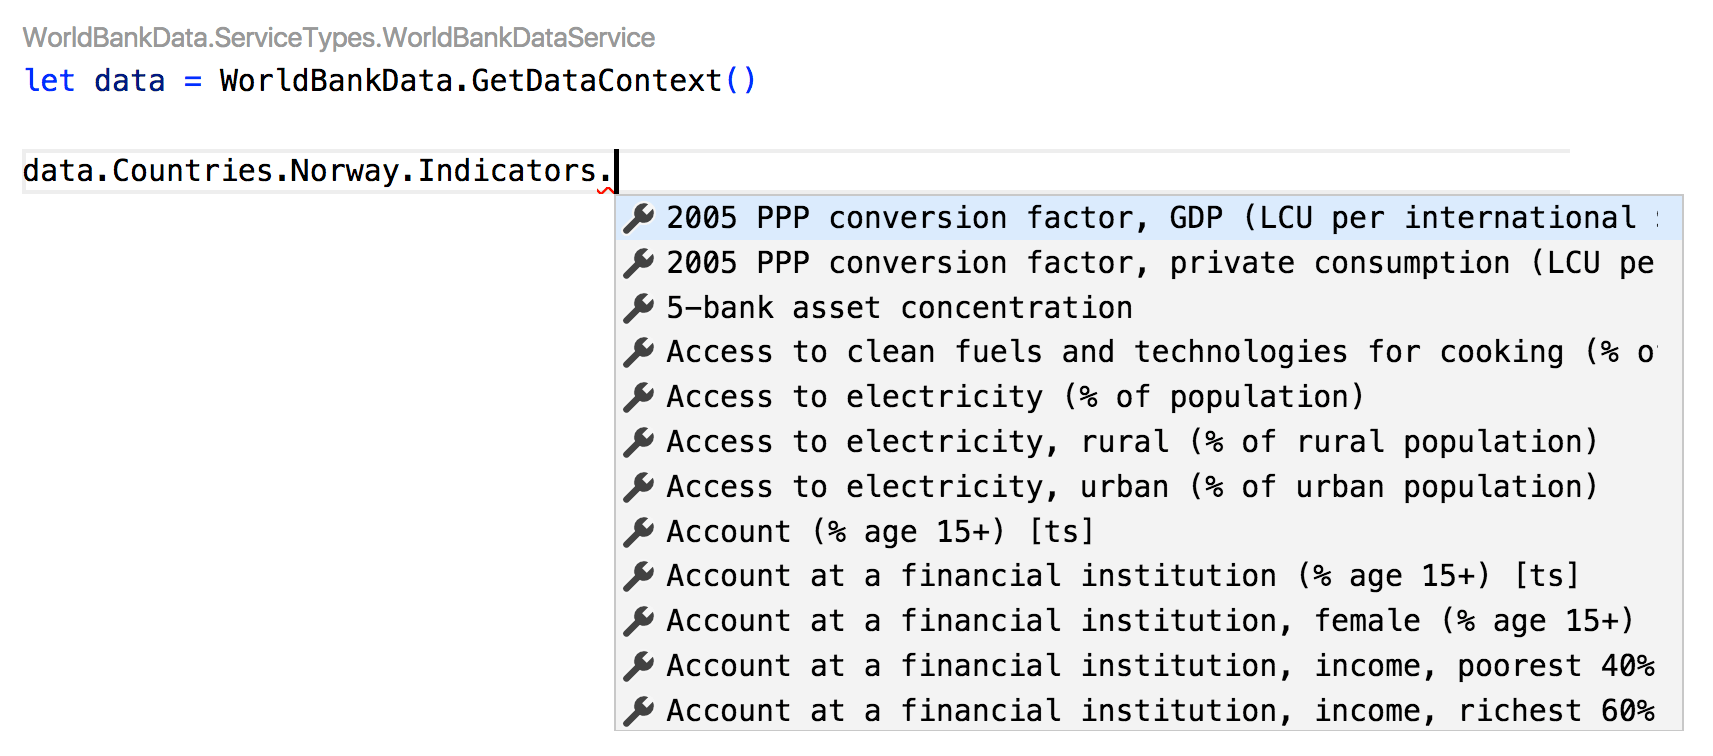
\includegraphics[width=0.8\textwidth]{images/worldbank_autocomplete}
\end{center}
\hspace*{-1.5in} % To get rid of some weird bottom margin
\caption{Autocomplete from the WorldBank type provider}
\label{fig:worldbank-autocomplete}
\end{figure}

A good example of a type provider which makes use of this functionality is the WorldBank type provider in \fsharpdata. As the name suggests, it provides access to the World Bank data catalog via its web API. Figure~\ref{fig:worldbank-autocomplete} shows a screenshot of the kind of autocomplete that is available when using the type provider. Having such functionality makes it quick and easy to dive into the data, and it would be very hard, or impossible, to replicate without some sort of strategy for only generating what is necessary.

While thunks as parts of generated types is clearly a very powerful feature, many of F\#s type providers are not reliant on it. If it is feasible to have all the necessary data available at once, and the generated type is not too large, delayed production of the code is not required. For example the ‹JsonProvider› from \fsharpdata\ which creates a single type hierarchy from a limited set of samples, does not need thunks. In other words, something like ‹JsonProvider› \emph{should} be possible in Rust. In chapter~\ref{chap:project-presentation} I will show how I have attempted to achieve this, but let us first look at the advantages and disadvantages of the type providers it is inspired by.

\subsection{Advantages of F\#s type providers}

% "Type checking" external resources
The most significant benefit of type providers is that they enable type-safe access to external resources, significantly improving type checking for sections of code using data from a type provider.

% Explorative programming / Tooling help
As mentioned, such type-safe access can also be achieved by manually writing the custom types, but the ease of use of a type provider makes it very easy to add a new external resource and start experimenting. Not only is the barrier of having to write boilerplate code reduced or removed, but type information gleaned through e.g. autocomplete facilitates exploration of the resource.

When working with external data, the code we write encode our assumptions about the data we are working with. E.g. if I have parsed some data into a variable ‹p› and I write code like ‹let real_name: String = p.name›, the code encodes my assumptions that the data has a field with the name ‹name›, and that said field is a string. When the types are in sync with the external data the type checking will thus check that our assumptions match the actual structure of the data. Additionally, the type checking will \emph{only} check the assumptions we state through our use of the data, which are likely to be the ones we care about.

% Detect API changes
Since these assumptions are re-checked when we re-compile this can help us not just when our assumptions change, but also when the things we are making assumptions about change. In this way a type provider like ‹JsonProvider› can help alert us about changes to remote resources while we are developing or in a continuous  integration setting.

% Encoding of otherwise impractical/impossible types
The most advanced type providers can thanks to the delayed evaluation of AST encode information that would otherwise be entirely impractical to otherwise encode in the type system. We will be hard pressed to recreate this in Rust since we will not have access to delayed evaluation, but there may be other ways that we may be able to make different trade-offs and thus explore new possibilities.

\subsection{Disadvantages of F\#s type providers}
\label{sec:disadvantages-of-type-providers}

While F\#s type providers have significant advantages, they also have some disadvantages. Type providers are essentially a code generation tool. However, type providers do not give the user access to the generated code. For type providers that use thunks, it is of course not a real option to generate the full code to be able to show it, as the \say{full} code could in fact be infinite. And if you just show the code that is already forced by the program usage, no new information is provided.

% Understanding code you cannot see

Since the difference between type providers that use delayed evaluation and those that don't is completely abstracted away from the users of the type providers, this means that there is no option to look at the generated code to understand what is going on and to inspect the structure of the parsed data. While some of the same understanding can be achieved by looking at the autocomplete suggestions it is often easier to understand the structure by looking at the actual types.

% Migration path

No access to the generated code also causes a certain amount of lock-in. Without access to the code, trying to migrate a project using type providers to manually written types forces a complete rewrite of the types provided by the type provider. In the case of parsing JSON and generating types from it there are many trade-offs that have to be made, and thus there might be reasons for such a migration as a project develops. I will come back to these trade-offs in section~\ref{sec:configurability}.

% Network access
A completely different issue with certain type providers is that they provide the greatest benefit with concern to the type checking when verifying the use of an external resource. However, if access to this external resource requires network access, this causes the compilation of the program to require network access for every build. Sometimes requiring network access to build is not a big concern, but other times it can be a big annoyance or even be completely out of the question.

% Build can break without code changes
Another concern many people have with type providers is that since the type checking checks if the code matches the data, the build can break if the structure of the data changes. In other words, the advantage of having our assumptions checked by the type checking also means that the build can break without any changes to the things we manage with version control. Such breakage runs contrary to the concept of reproducible builds which is a very common goal for build systems. One may counter that an external data source like an API is part of the system when it is used in a program, and as such a build failure is the correct behavior, but it is nevertheless a contentious issue.

While these very real concerns are not something that dissuade us from pursuing the significant benefits that type providers can give us, we should at the same time keep them in mind as we go forward.
